\begin{frame}{\tcii{} Policy search}
    \onslide<2->{
    \begin{center}
      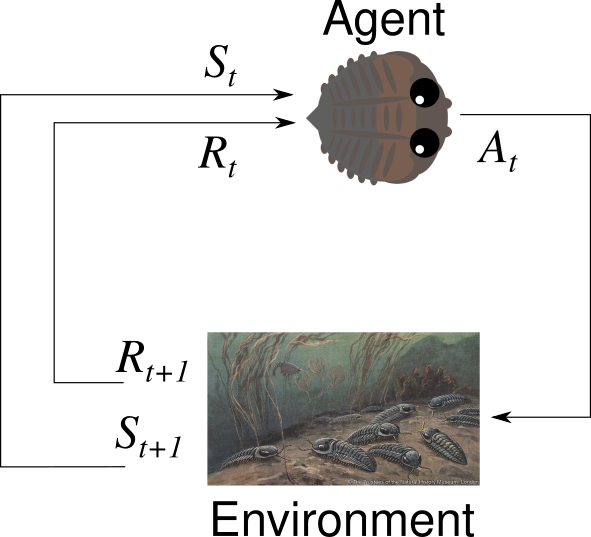
\includegraphics[width=7cm]{images/misc/erl.png}\\
      \small \url{https://github.com/d9w/evolution/blob/master/imgs/erl.png}
    \end{center}
    }
\end{frame}

\begin{frame}{\tcii{} Neural networks}
    \begin{center}
      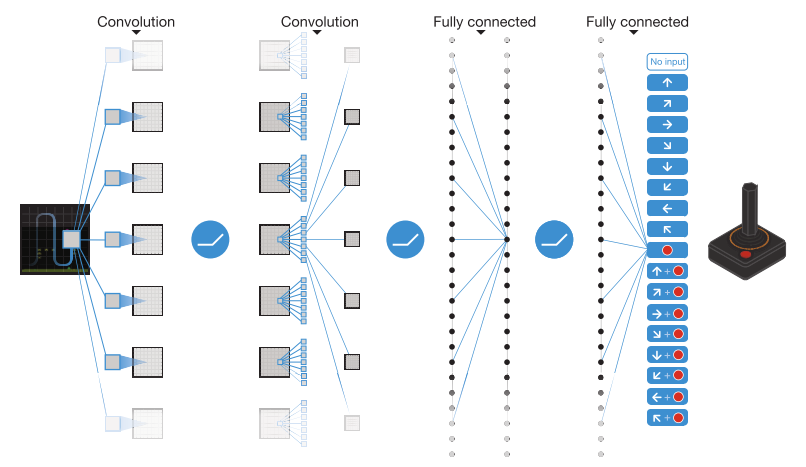
\includegraphics[width=8cm]{images/misc/dqn.png}\\
      \small Neural Network used in Deep Q Networks \cite{mnihHumanlevelControlDeep2015}
    \end{center}
\end{frame}

\begin{frame}{\tcii{} \es}
    \begin{center}
      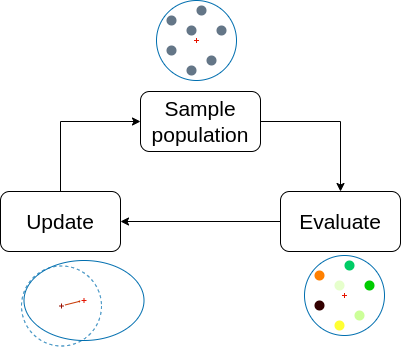
\includegraphics[width=6cm]{images/misc/es.png}\\
      \small Evolution Strategy steps
    \end{center}
\end{frame}

\begin{frame}{\tcii{} Variants of \es}
    \onslide<1->{
    \begin{block}{Evolution Strategies}
        \begin{columns}
            \begin{column}{0.45\linewidth}
                \begin{itemize}
                    \item ($\mu , \lambda$) ES
                    \item \snes
                    \item Canonical ES 
                    \item OpenAI ES
                \end{itemize}
            \end{column}
            \begin{column}{0.45\linewidth}
                \begin{itemize}
                    \item \cmaes
                    \item \xnes
                    \item Cross-Entropy Method
                    \item Augmented Random Search
                \end{itemize}
            \end{column}
        \end{columns}
    \end{block}
    }
    \onslide<2->{   
    \begin{block}{Neuroevolution for policy search}
        \begin{itemize}
            \item large dimensions (1.6 $.10^6$ parameters)
            \item expensive evaluation 
        \end{itemize}
    \end{block}
    }
    
\end{frame}

\begin{frame}{\tcii{} \berl{}}

    \begin{block}{Reproduction settings}
        Reproducing \canonical{} \canonicalpaper{} and \openaies{} \openaipaper{} on the Arcade Learning Environment.
    \end{block}
    
    \begin{center}
        \begin{figure}
            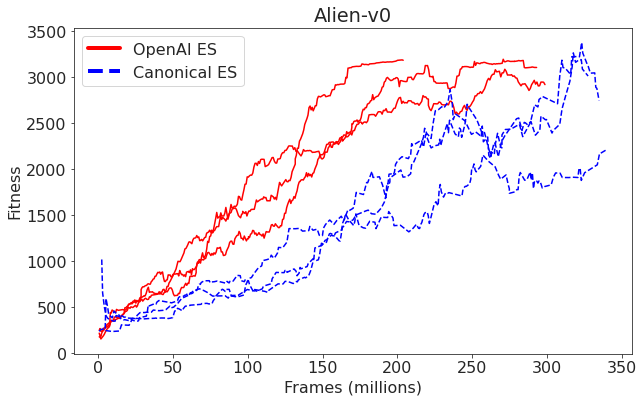
\includegraphics[width=7cm]{images/BERL/Alien-v0.png}
            \caption{Evolution of \canonical{} and \openaies{} on Alien with 800 CPUh compute budget}
        \end{figure}
    \end{center}

\end{frame}